%!TEX root = ../uwo.tex

\begin{frame}[plain,noframenumbering]
	\centering
	\vspace*{2.6cm}
	\Huge \colorit{Part II}
	\vskip 20pt
	\Large Persistence homology
\end{frame}

\begin{frame}{Points clouds and multi-scale approximation}
	\pause
	Data sets are often encountered as point clouds in $\R^n$.

	\pause
	\begin{center}
		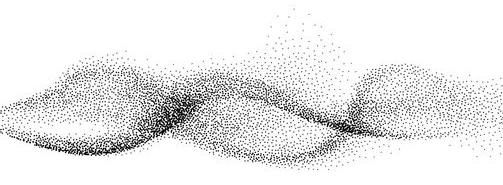
\includegraphics[scale=.4]{aux/point_cloud_cropped}
	\end{center}

	\pause
	Their underlying probability distribution is concentrated on a subspace.

	\medskip\pause
	Use \colorit{distance parameter} to approximate it with simplicial complexes.
	\medskip
	\begin{center}
		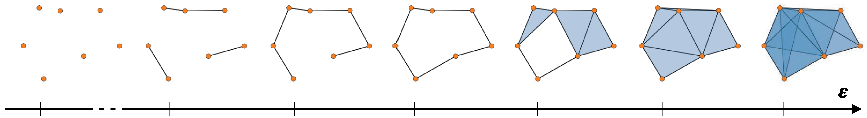
\includegraphics[scale=.7]{aux/vietoris-rips}
	\end{center}

	\vskip-15pt
	\[
	X_{0} \subset X_{1} \subset\dots\subset X_{n}
	\]
\end{frame}

\begin{frame}{Persistence homology}
	\pause
	Applying a homology functor (over a field)
	\[
	H_d(X_0) \to H_d(X_1) \to\dots\to H_d(X_n)
	\]
	get a \colorit{persistence module}, i.e. a diagram of vector spaces.

	\pause\bigskip
	The way dimensions fit together defines the \colorit{barcode}.
	\begin{center}
		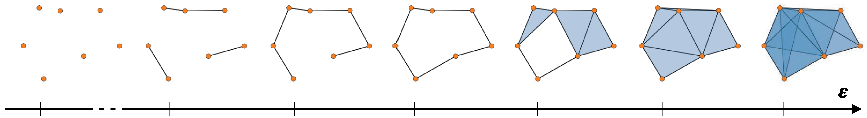
\includegraphics[scale=.7]{aux/vietoris-rips}
		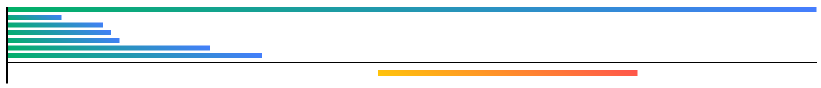
\includegraphics[scale=.6]{aux/betti}
	\end{center}

	\pause\smallskip
	\colorit{Stability}: The passage from point clouds to barcodes is Lipschitz
	\[
	d_{GH}(\fX, \fX') \leq \bars{B_{\fX}, B_{\fX'}}.
	\]

	\pause
	\colorit{Computability}: Based on matrix reduction algorithms
	\[
	\sim O(n^3).
	\]
\end{frame}

\begin{frame}{Exemplar - Nanoporous materials (Lee et al.)}
	\pause
	\textcolor{pblue}{Comparing geometries} \\
	directly, impossible, \\
	over 3M structures.

	\begin{textblock*}{4cm}(5.4cm,1.5cm)
		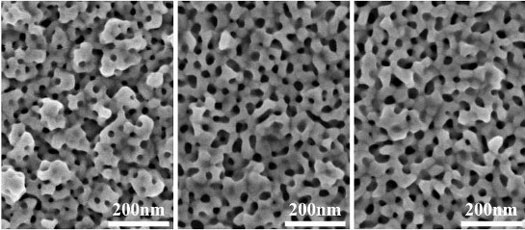
\includegraphics[scale=.28]{aux/real_material}
	\end{textblock*}

	\pause\vspace*{2cm}
	\textcolor{pblue}{Comparing Barcodes} \\
	is done fast \\
	and faithfully \\
	by stability.

	\vspace*{-2.3cm}\hspace*{3.8cm}
	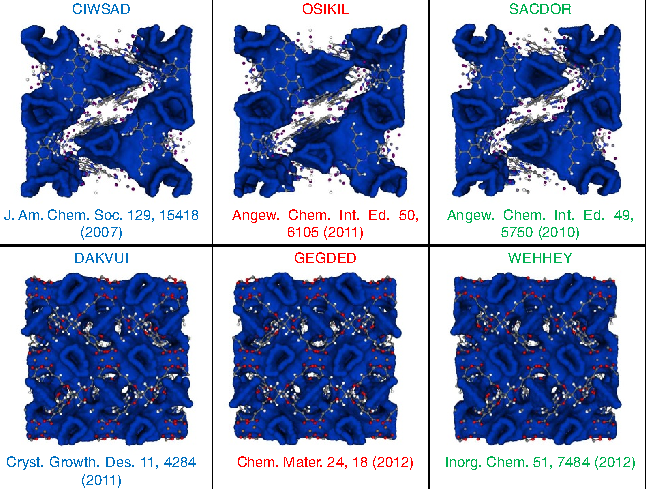
\includegraphics[scale=.6]{aux/nanoporous}
\end{frame}

\begin{frame}{Bringing barcodes to machine learning}
	\pause
	Integration of persistence algorithms into scikit-learn.
	\vskip 10pt
	
\includegraphics[scale=.31]{aux/giotto}
\end{frame}
